\section{Project Implementation and Outcomes}
\label{sec:implementation}

This section covers what was built and how it works. Where things changed from the original plan, the text explains why.

\subsection{Architecture Evolution}

The original design called for a Python backend with FastAPI and a Next.js frontend. Two weeks in, this changed: every data structure crossing the API boundary had to be defined twice, and mismatches caused silent runtime failures. Switching everything to TypeScript (SE3) took four days but removed a whole category of bugs. The \texttt{shared-types} package now defines every interface once, and the compiler catches mismatches at build time.

\subsection{Monorepo Structure}

The codebase uses Turborepo to manage three applications and one shared package (SE12):

\begin{table}[H]
\centering
\begin{tabular}{|l|l|l|}
\hline
\rowcolor{gray!20} \textbf{Package} & \textbf{Technology} & \textbf{Purpose} \\
\hline
\texttt{apps/service} & Express.js, TypeScript & Backend API: orchestration, template \\
 & & analysis, content planning, slide building \\
\hline
\texttt{apps/web} & Next.js, React, TypeScript & Web frontend: PB management, \\
 & & slide preview, generation trigger \\
\hline
\texttt{apps/powerpoint-addin} & Vite, React, TypeScript, & PowerPoint taskpane: in-editor \\
 & Office.js & generation and AI-assisted editing \\
\hline
\texttt{packages/shared-types} & TypeScript & Shared interfaces, enums, and \\
 & & type definitions across all apps \\
\hline
\end{tabular}
\caption{Monorepo Package Structure}
\label{tab:monorepo}
\end{table}

Figure~\ref{fig:dashboard} shows the web app dashboard after login.

\begin{figure}[H]
\centering
\screenshot{screenshots/web-app/04-dashboard.png}
\caption{Web app dashboard showing pitch book counts, recent generation history, and sidebar navigation.}
\label{fig:dashboard}
\end{figure}

\subsection{Orchestration Layer}

The orchestrator runs each stage in sequence and stays thin: each service module handles its own domain. Figure~\ref{fig:orchestrator} shows the full pipeline. If data retrieval fails, it passes an empty object to the content planner rather than aborting. The orchestrator passes the full template schema to GPT-4o rather than a summary, because early versions with only layout names produced worse output.

\begin{figure}[H]
\centering
\begin{tikzpicture}[
  step/.style={draw, rounded corners, minimum width=3cm, minimum height=0.8cm, align=center, font=\small, fill=blue!12},
  fail/.style={draw, rounded corners, minimum width=2.2cm, minimum height=0.6cm, align=center, font=\scriptsize, fill=red!10, dashed},
  data/.style={draw, rounded corners, minimum width=2.2cm, minimum height=0.6cm, align=center, font=\scriptsize, fill=gray!15},
  arr/.style={->, thick},
]

% Steps - vertical flow
\node[step] (validate) at (0, 0) {Validate Input};
\node[step] (extract) at (0, -1.5) {Extract Template};
\node[step] (retrieve) at (0, -3) {Retrieve Data};
\node[step] (plan) at (0, -4.5) {Plan Content (GPT-4o)};
\node[step] (build) at (0, -6) {Build Slides};
\node[step] (preview) at (0, -7.5) {Generate Previews};
\node[step] (store) at (0, -9) {Store Result};

% Arrows
\draw[arr] (validate) -- (extract);
\draw[arr] (extract) -- (retrieve);
\draw[arr] (retrieve) -- (plan);
\draw[arr] (plan) -- (build);
\draw[arr] (build) -- (preview);
\draw[arr] (preview) -- (store);

% Side outputs
\node[data] (schema) at (4, -1.5) {Template\\Schema};
\draw[arr] (extract) -- (schema);
\draw[arr] (schema) |- (plan);

\node[data] (findata) at (4, -3) {Financial\\Data / \{\}};
\draw[arr] (retrieve) -- (findata);
\draw[arr] (findata) |- (plan);

\node[data] (contentplan) at (4, -4.5) {Content\\Plan (JSON)};
\draw[arr] (plan) -- (contentplan);
\draw[arr] (contentplan) |- (build);

\node[data] (pptx) at (4, -6) {.pptx File};
\draw[arr] (build) -- (pptx);
\draw[arr] (pptx) |- (preview);

% Failure paths
\node[fail] (faildata) at (-4, -3) {API failure?\\Pass empty \{\}};
\draw[->, dashed, red!60!black] (retrieve.west) -- (faildata);

\node[fail] (failplan) at (-4, -4.5) {Zod invalid?\\Fallback plan};
\draw[->, dashed, red!60!black] (plan.west) -- (failplan);

\end{tikzpicture}
\caption{Orchestration pipeline. Each stage passes its output to the next. Dashed paths show graceful failure handling: data retrieval passes an empty object on API failure, and the content planner falls back to a generic plan if Zod validation fails.}
\label{fig:orchestrator}
\end{figure}

\subsection{Deck Layouts and Colour Themes}

The system ships with seven deck layouts (Company Overview, Investor Pitch, Market Update, Transaction Summary, Industry Overview, Fundraising Deck, Due Diligence) and eight built-in colour themes. The layouts are hardcoded because IB slide sequences are standard across the industry. The visual style is customisable: users pick a theme or upload a bank's own template file. When a template is uploaded, the analyser extracts that bank's exact colours, fonts, and layout positions, and the slide builder applies them to whichever layout the user picks. Figure~\ref{fig:new-pitchbook} shows the creation form.

\begin{figure}[H]
\centering
\screenshot{screenshots/web-app/06-new-pitchbook.png}
\caption{New pitch book creation form. The user selects a deck layout, colour theme, and enters company details before generating.}
\label{fig:new-pitchbook}
\end{figure}

\subsection{Core Pipeline}

The generation pipeline follows the design from Section~\ref{sec:research-design}, implemented as a chain of service modules within the Express backend. Each stage is a separate TypeScript module with a defined input/output contract. Development followed a pattern: build the simplest version, test it against real templates, identify the failure mode, and fix it.

\subsubsection{Template Analysis}

The template analyser went through three iterations, each driven by a specific failure in the previous version (SE4).

\textbf{Iteration 1: PptxGenJS only.} The first attempt used PptxGenJS for both reading and writing slides. PptxGenJS can create slides from scratch but has no API for reading existing .pptx files. The only option was to generate new slides and hope the styling matched. It did not. Colours were wrong, placeholder positions were guessed rather than measured, and the output looked nothing like the input template. This approach was scrapped after two days.

\textbf{Iteration 2: JSZip + xml2js (raw XML parsing).} PowerPoint files are ZIP archives containing Office Open XML documents. XML (Extensible Markup Language) is a text-based format that stores data in nested tags, similar to HTML but with custom tag names defined by the application. A .pptx file contains dozens of XML files that describe every slide, shape, colour, and font in the presentation. JSZip opens the archive, and xml2js parses the XML inside. This gave direct access to every property: colours from \texttt{ppt/theme/theme1.xml}, layouts from \texttt{ppt/slideLayouts/}, and placeholder positions from shape definitions. The approach worked but came with a problem. PowerPoint's OOXML specification stores measurements in English Metric Units (EMU), where one inch equals 914,400 EMU. Colours can be stored as hex values, theme references (\texttt{accent1}), or system colour names. Placeholder types use numeric codes, but custom placeholders have no type attribute at all. Each of these required manual parsing and conversion logic.

\textbf{Iteration 3: heuristics and fallbacks for analysis.} Testing against real corporate templates exposed gaps in the raw XML approach. Custom placeholders with no type attribute made up roughly 30\% of all placeholders in the test set. The analyser added position-based heuristics: a placeholder in the top 15\% of the slide with large font settings is classified as a title, even without a type code. A wide placeholder in the bottom half with small fonts is treated as body text. This brought classification accuracy to 93\% across test templates. When parsing fails entirely (corrupted file, unusual XML structure), the analyser falls back to professional defaults: a navy and gold colour scheme with standard IB layout patterns.

\vspace{0.5em}\filbreak
\begin{lstlisting}[language=JavaScript, caption=Template extraction core logic (simplified)]
async function analyseTemplate(buffer: Buffer): Promise<TemplateSchema> {
  const zip = await JSZip.loadAsync(buffer);

  // Parse theme for colour palette
  const themeXml = await zip.file('ppt/theme/theme1.xml')?.async('string');
  const theme = await parseStringPromise(themeXml);
  const colours = extractColourScheme(theme);

  // Parse each slide layout
  const layouts: SlideLayout[] = [];
  for (const [path, file] of Object.entries(zip.files)) {
    if (path.match(/ppt\/slideLayouts\/slideLayout\d+\.xml/)) {
      const xml = await file.async('string');
      const parsed = await parseStringPromise(xml);
      layouts.push(extractLayout(parsed, colours));
    }
  }

  return { colours, fonts: extractFonts(theme), layouts };
}
\end{lstlisting}

Each version failed in a specific, observable way, and the fix was targeted rather than speculative (SE4). The unit tests grew alongside: the third iteration added edge-case tests for missing themes, custom placeholders, and corrupted archives (SE5).

The analyser reads layout information from the slide master. Figure~\ref{fig:template-master} shows the master view for a sample template. Each thumbnail on the left is a slide layout. The master defines where placeholders go, what fonts to use, and what the background looks like. The analyser reads these from the \texttt{ppt/slideLayouts/} directory and records the placeholder types, positions, and styling.

\begin{figure}[H]
  \centering
  \screenshot{screenshots/templates/master.png}
  \caption{Slide master view showing the available layouts for a template. Each layout defines placeholder positions, fonts, and background styling that the generation pipeline inherits.}
  \label{fig:template-master}
\end{figure}

\subsubsection{Content Planning with GPT-4o}

The content planner sends user parameters and the extracted template schema to GPT-4o, requesting a structured content plan. Getting the prompt right took several iterations. The first version produced slides full of generic phrases like ``strong market position'' and ``leading industry player'' with no company-specific detail. Adding a rule banning generic phrasing helped, but the slides were still sparse, with two or three short bullet points per slide. The final system prompt (Code~\ref{lst:system-prompt}) sets minimum content density per slide type and provides examples of good versus bad output. It also instructs the model to write as a senior Managing Director rather than a generic assistant, which consistently produced more specific, data-driven language.

\vspace{0.5em}\filbreak
\begin{lstlisting}[language=JavaScript, caption=Content planner system prompt excerpt (from pitchbook-content.prompt.ts), label=lst:system-prompt]
export const SYSTEM_PROMPT = `You are a senior Managing Director at
Goldman Sachs creating investment banking pitch books.

CRITICAL RULES:
1. ALL financial data MUST use the EXACT numbers provided in the
   user message. NEVER fabricate numbers.
2. Every chart MUST have a "data" array with real numbers.
3. Content must be deeply specific to the company. Mention their
   actual products, markets, competitors, recent events.
4. Write like a real IB analyst: precise, data-driven, no fluff.
5. NEVER write generic phrases like "leading company in its sector"
   or "strong market position". Be SPECIFIC.

CONTENT DENSITY:
- Every Content Slide MUST have at least 5-7 bullet points.
- Every bullet point must be a FULL SENTENCE with specific data.
  BAD: "Strong revenue growth".
  GOOD: "Revenue grew 61% YoY to 130.5B in FY2024, driven by
  Data Center segment expansion to 115.2B."
- Financial Tables should have 4-5 years of data with 5+ rows.

You MUST return JSON in EXACTLY this format:
{ "title": "...", "narrative_arc": "...", "slides": [...] }`;
\end{lstlisting}

Getting valid structured output was the main challenge (SE1). \textcite{shorten2024} found an average JSON success rate of 82.55\% across LLM benchmarks. GPT-4o occasionally wraps responses in unexpected envelope objects. The content planner handles this with an unwrapping step before Zod \parencite{zod2024} schema validation. If validation fails, a hardcoded fallback plan keeps generation going. Across 12 evaluation runs, all produced valid JSON without needing the fallback. The prompt includes retrieved financial data so the LLM places real numbers rather than fabricating them.

\vspace{0.5em}\filbreak
\begin{lstlisting}[language=JavaScript, caption=Content plan validation with Zod (from pitchbook-content.schema.ts)]
const contentBlockSchema = z.object({
  type: z.enum(['heading', 'paragraph', 'bullet_list',
                'table', 'chart', 'metric']),
  content: z.any(),
});

const slideSchema = z.object({
  index: z.number().optional().default(0),
  title: z.string(),
  layout: z.string().optional().default('Content Slide'),
  talking_points: z.array(z.string()).optional().default([]),
  data_requirements: z.array(z.string()).optional().default([]),
  content_blocks: z.array(contentBlockSchema).optional().default([]),
});

const contentPlanSchema = z.object({
  title: z.string(),
  narrative_arc: z.string().optional().default(''),
  slides: z.array(slideSchema),
});

function parseContentPlan(raw: unknown): ContentPlanOutput {
  return contentPlanSchema.parse(raw);
}
\end{lstlisting}

\subsubsection{Slide Building}

The system has two slide building paths, selected by whether the user uploaded a template (SE10).

\textbf{Default mode} uses PptxGenJS to generate slides from scratch with a built-in theme selected by pitch book type. Theme colour references (\texttt{accent1}, \texttt{dk1}) are resolved to hex values before applying, since PptxGenJS has no theme colour system.

\textbf{Template mode} clones the template's actual slides and replaces placeholder text using regex on the raw XML. Figure~\ref{fig:template-original} shows a sample template with 14 slides. The builder parses each slide's \texttt{.rels} file to find its layout name, then for each content plan slide, picks the best-matching template slide. It finds each \texttt{<p:sp>} shape containing a \texttt{<p:ph>} (placeholder) element and replaces the \texttt{<p:txBody>} content while preserving the original \texttt{<a:bodyPr>}, \texttt{<a:lstStyle>}, and \texttt{<a:rPr>} (font, size, colour) via regex extraction. The result: generated text comes out in the template's own font, size, and colour.

This approach uses regex on the raw XML rather than xml2js round-tripping, which corrupted OOXML namespace declarations and produced files that Office.js rejected. The builder also injects \texttt{<a:normAutofit>} to auto-shrink overflowing text and truncates content per placeholder type (120 characters for titles, 7 bullets at 150 characters each, 500 for body text).

\begin{figure}[H]
  \centering
  \screenshot{screenshots/templates/template.png}
  \caption{Original template with 14 slides across different layout types, each with a consistent brown and gold visual style.}
  \label{fig:template-original}
\end{figure}

\begin{figure}[H]
  \centering
  \screenshot{screenshots/templates/result.png}
  \caption{Generated output for Meta Platforms using the template from Figure~\ref{fig:template-original}. The 11 slides inherit the template's Felix Titling font, brown background, and gold accents. The add-in taskpane (right) shows slides were inserted directly into PowerPoint.}
  \label{fig:template-result}
\end{figure}

\subsubsection{Data Retrieval}

The data retrieval service pulls financials from Yahoo Finance (\texttt{yahoo-finance2}) and SEC EDGAR (K5). Yahoo Finance provides market cap, trailing revenue, share price, historical income statements, balance sheet data, and cash flow summaries. SEC EDGAR provides recent 10-K (annual), 10-Q (quarterly), and 8-K (material event) filing summaries for US-listed companies. All of this data is injected directly into the GPT-4o prompt so the model places real numbers rather than generating its own. This is the architectural decision behind the 100\% data accuracy result in Section~\ref{sec:evaluation}. The LLM never estimates financial figures because it never needs to. Responses are cached for 24 hours to avoid hitting rate limits and to speed up repeated generations for the same company. The cache uses an in-memory store rather than a database because the data changes daily and stale cache entries are acceptable for a first draft.

If an API call fails, the service returns graceful null values rather than aborting. The content planner receives an empty data object and generates slides without financial figures, producing a structural draft that the analyst fills in manually. This design means a Yahoo Finance outage degrades output quality but never blocks generation entirely. The abstract interface behind both data sources (Section~\ref{sec:methodology}) means switching to a licensed provider like Bloomberg or Refinitiv would require changing one module without touching the rest of the pipeline.

\subsubsection{Slide Preview Generation}

The system uses LibreOffice in headless mode to convert .pptx to PDF, then \texttt{pdftoppm} to render each page as a PNG at 150 DPI. Previews are uploaded to Supabase Storage with signed URLs and displayed in the web frontend's slide viewer. The pipeline runs asynchronously after slide assembly completes, so the .pptx file is available immediately while previews generate in the background.

Neither this pipeline nor the add-in below were in the original design. Both emerged from usability problems found during implementation. The web app originally showed only a download link for the generated file. Without visual previews, users had to open the file in PowerPoint to see what was generated, which added friction and made the web interface feel disconnected from the output. Adding preview images turned the web app into a useful management interface even after the add-in became the primary generation tool.

\subsection{From Web-Only to Add-in: The Product Pivot}
\label{sec:pivot}

The original plan was a web-only application where the user would fill in a form and receive a .pptx download. That design assumed the generated deck would be close enough to final that a download-and-open step was acceptable. It was not.

Pitch books are never finished after the first draft. Analysts reword bullet points, swap slide ordering, adjust font sizes, reposition charts, and tweak colours to match the managing director's preferences. Every deck goes through multiple rounds of revision. A web-only tool that produces a download link ignores this reality.

Two options existed for supporting editing. The first was building a slide editor into the web app, which would mean recreating a subset of PowerPoint in the browser. Text editing alone needs drag-to-reposition, resize handles, font pickers, and layer ordering. Tools like Google Slides and Canva have entire teams working on their browser editors. Attempting this in a 13-week project would have consumed the remaining timeline and produced a worse experience than PowerPoint itself. A natural language interface for spatial editing (``move the title left'', ``change the chart colours'') would be equally frustrating. Telling a chatbot to nudge elements until they look right takes longer than dragging them with a mouse.

The better path was to work inside PowerPoint rather than against it. PowerPoint already handles slide editing well, and it supports add-ins, which are small web applications that run in a taskpane and communicate with the active presentation via Office.js. The system's value is not in replacing that editor but in removing the blank-page problem.

This led to the v2 architecture. The add-in handles generation and insertion directly into the active presentation. The analyst stays in PowerPoint for the full workflow. The web app shifted to a management layer for storing pitch books, displaying previews, tracking history, and hosting the AI chat. Future features like RAG search (FR15, deferred) would also sit in the web app, since browsing a document library does not belong in a PowerPoint taskpane.

The pivot validated the iterative methodology. A waterfall approach would have delivered the planned web-only system and missed the usability problem entirely. The working prototype in week 7 made the friction visible and measurable, and the modular architecture meant the add-in could reuse the same backend and shared types without duplicating pipeline logic (SE7, SE8).

\subsection{PowerPoint Add-in}
\label{sec:addin}

The add-in is a taskpane built with Office.js that runs inside PowerPoint, communicating with the same Express backend as the web app.

\begin{figure}[H]
\centering
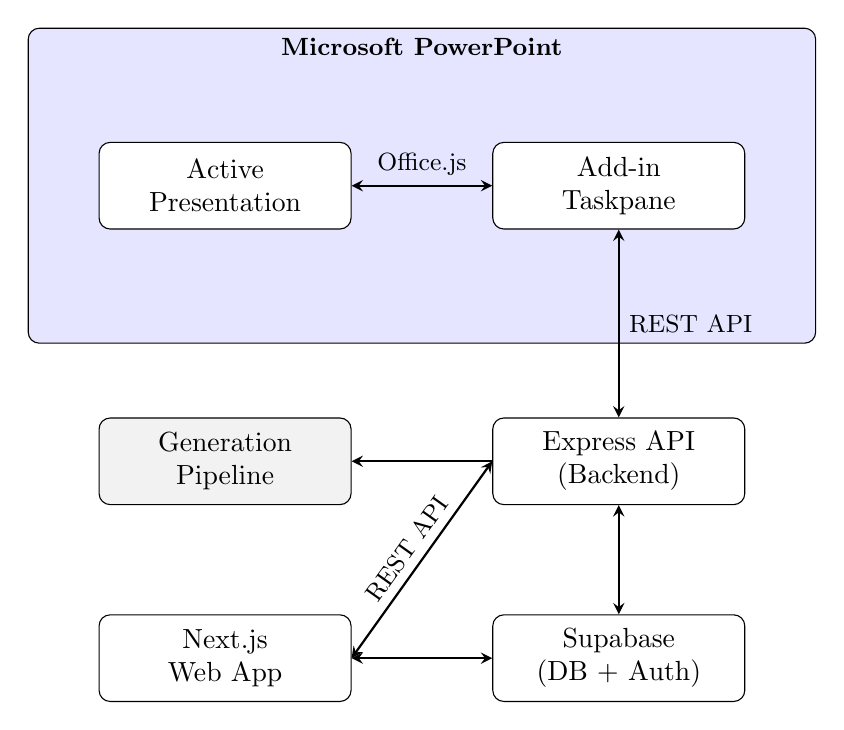
\begin{tikzpicture}[
    box/.style={draw, rounded corners, minimum width=3.2cm, minimum height=1.1cm, align=center},
    arr/.style={->, thick, >=stealth},
    darr/.style={<->, thick, >=stealth}
]
% PowerPoint container
\node[box, fill=blue!10, minimum width=10cm, minimum height=4cm] (ppt) at (0, 5) {};
\node[anchor=north, font=\bfseries\small] at (0, 7) {Microsoft PowerPoint};

% Inside PowerPoint
\node[box, fill=white] (ap) at (-2.5, 5) {Active\\Presentation};
\node[box, fill=white] (addin) at (2.5, 5) {Add-in\\Taskpane};
\draw[darr] (ap) -- node[above, font=\small] {Office.js} (addin);

% Backend row
\node[box] (api) at (2.5, 1.5) {Express API\\(Backend)};
\node[box, fill=gray!10] (gen) at (-2.5, 1.5) {Generation\\Pipeline};

% Add-in to backend
\draw[darr] (addin) -- node[right, font=\small] {REST API} (api);

% API to pipeline
\draw[arr] (api) -- (gen);

% Bottom row
\node[box] (web) at (-2.5, -1) {Next.js\\Web App};
\node[box] (db) at (2.5, -1) {Supabase\\(DB + Auth)};

% Web to API - straight diagonal with label
\draw[darr] (web.east) -- node[above, font=\small, sloped] {REST API} (api.west);

% API to DB
\draw[darr] (api) -- (db);

% Web to DB
\draw[darr] (web) -- (db);
\end{tikzpicture}
\caption{System architecture with PowerPoint Add-in. The add-in and web app share the same backend and database. A pitch book generated in either interface is stored centrally and accessible from both.}
\label{fig:addin-architecture}
\end{figure}

Because both the web app and the add-in connect to the same Express backend and Supabase database, a pitch book generated in either interface appears in both. An analyst can start a generation from the web app's creation form, and the resulting deck will be available in the add-in's pitch book list when they open PowerPoint. The reverse also works. This means the two interfaces are not separate tools but two views of the same data, each suited to a different task.

\begin{figure}[H]
\centering
\screenshot{screenshots/add-in/1-addin-full.png}
\caption{PowerPoint with the add-in taskpane open. Generated slides appear in the slide panel on the left, and the AI chat input sits at the bottom of the taskpane.}
\label{fig:addin-taskpane}
\end{figure}

The \texttt{insertSlidesFromBase64()} API pushes the generated .pptx directly into the active presentation. The web app became a management interface for browsing pitch books. Both applications share the same backend (K5).

\begin{figure}[H]
\centering
\screenshot{screenshots/web-app/05a-pitchbook-deck-layout.png}
\caption{Pitch book viewer showing slide preview, thumbnail navigation, and AI chat panel.}
\label{fig:pitchbook-viewer}
\end{figure}

\subsection{AI Chat Assistant}
\label{sec:ai-chat}

The pitch book viewer includes an AI chat panel (visible in Figure~\ref{fig:pitchbook-viewer}) that lets users request slide changes in plain English. An analyst might type ``make the executive summary more focused on the data centre segment'' or ``add a bullet about the recent acquisition''. The chat runs on GPT-4o-mini, which is cheaper and faster than GPT-4o. Structured output is not required here since the model returns natural language advice rather than JSON. The system prompt includes each slide's title and layout type so the model can reference specific slides in its response. Messages are stored in a \texttt{chat\_messages} table, preserving history across sessions.

The chat is advisory. The assistant provides instructions and suggested text, but the user applies the edits. Office.js can modify slides programmatically, so automatic application is technically possible. The advisory boundary was drawn deliberately to keep the analyst in control of every change. In a regulated industry where every word on a client-facing slide carries professional liability, automatic edits without human approval would introduce risk that outweighs the convenience. This is consistent with the HITL design principle from Section~\ref{sec:introduction}.

\subsection{Authentication and Session Management}

Supabase Auth handles user authentication across both applications. The Express backend acts as the single auth source, checking session cookies on every request (SE1). The add-in runs inside an Office.js iframe whose WebView enforces stricter cross-origin rules than a standard browser tab. Cookies are blocked by default, and Safari's Intelligent Tracking Prevention actively strips third-party cookies. This required \texttt{SameSite=None; Secure} cookie attributes and explicit CORS configuration, which was one of the harder debugging problems in the project because failures were silent (the cookie was simply absent).

\subsection{Testing}

The project uses three levels of testing: unit tests for individual modules, integration tests for service interactions, and end-to-end (E2E) tests for full user flows (SE5, SE11).

\subsubsection{Unit and Integration Tests}

Vitest \parencite{vitest2024} runs all unit and integration tests. It was chosen over Jest for native Vite module resolution and TypeScript support without extra setup. Turborepo runs all test suites in parallel via \texttt{turbo run test} and skips unchanged packages on repeat runs. Table~\ref{tab:test-coverage} shows what each test suite covers.

\begin{table}[H]
\centering
\begin{tabular}{|l|l|l|}
\hline
\rowcolor{gray!20} \textbf{App} & \textbf{Test File} & \textbf{What it Tests} \\
\hline
\texttt{apps/service} & \texttt{template-analyser.test.ts} & Colour, font, and layout extraction \\
 & & from known .pptx fixtures \\
\hline
\texttt{apps/service} & \texttt{content-planner.test.ts} & Zod validation rejects malformed \\
 & & LLM output, retries on failure \\
\hline
\texttt{apps/service} & \texttt{slide-builder.test.ts} & Output .pptx has correct formatting \\
 & & and valid XML structure \\
\hline
\texttt{apps/service} & \texttt{default-themes.test.ts} & Theme colours match specs when \\
 & & no template is uploaded \\
\hline
\texttt{apps/service} & \texttt{auth-middleware.test.ts} & Session validation, cookie parsing \\
\hline
\texttt{apps/web} & \texttt{api.test.ts} & API client calls and error handling \\
\hline
\texttt{apps/web} & \texttt{use-unsaved-changes.test.ts} & Hook warns before navigating away \\
\hline
\texttt{apps/powerpoint-addin} & \texttt{office-helpers.test.ts} & Office.js mock interactions \\
\hline
\texttt{apps/powerpoint-addin} & \texttt{component-logic.test.ts} & Form state and validation logic \\
\hline
\end{tabular}
\caption{Unit and Integration Test Coverage}
\label{tab:test-coverage}
\end{table}

Tests use \texttt{vi.mock()} to stub external dependencies (SE11) so they run without API keys or a database connection. Figure~\ref{fig:vitest-ui} shows the Vitest UI after a full run with all 134 tests passing.

\begin{figure}[H]
\centering
\screenshot{screenshots/tests/vitest.png}
\caption{Vitest UI showing all 14 test files and 134 tests passing across the three apps. The right panel displays the selected test's source code and can switch to console output on failure.}
\label{fig:vitest-ui}
\end{figure}

\subsubsection{E2E Tests}

Cypress \parencite{cypress2024} was chosen over Playwright for its low setup time with Next.js and built-in time-travel debugger. Tests run against a real Supabase backend with a test user account. Seven spec files cover the main user flows:

\begin{table}[H]
\centering
\begin{tabular}{|l|l|}
\hline
\rowcolor{gray!20} \textbf{Spec File} & \textbf{What it Tests} \\
\hline
\texttt{auth.cy.ts} & Login, logout, session persistence \\
\hline
\texttt{dashboard.cy.ts} & Dashboard loads, shows recent PBs \\
\hline
\texttt{pitchbooks.cy.ts} & Create, view, delete pitch books \\
\hline
\texttt{templates.cy.ts} & Upload and manage templates \\
\hline
\texttt{landing.cy.ts} & Public landing page renders correctly \\
\hline
\texttt{layouts.cy.ts} & Responsive layout across screen sizes \\
\hline
\texttt{settings.cy.ts} & User settings and preferences \\
\hline
\end{tabular}
\caption{Cypress E2E Test Specs}
\label{tab:cypress-specs}
\end{table}

Figures~\ref{fig:cypress-specs} to \ref{fig:cypress-failed} show the Cypress test runner in action.

\begin{figure}[H]
\centering
\screenshot{screenshots/cypress/specs.png}
\caption{Cypress test runner showing the E2E spec files grouped by feature area.}
\label{fig:cypress-specs}
\end{figure}

\begin{figure}[H]
\centering
\screenshot{screenshots/cypress/passed.png}
\caption{A passing Cypress test. The left panel shows each automated step (clicking elements, checking text), and the right panel shows the browser state at each step.}
\label{fig:cypress-passed}
\end{figure}

\begin{figure}[H]
\centering
\screenshot{screenshots/cypress/failed.png}
\caption{A failing Cypress test. The assertion expected either pitch book cards or an empty state message, but the data had not loaded yet when the check ran. This was a test logic error, not an application bug.}
\label{fig:cypress-failed}
\end{figure}

\subsubsection{CI/CD Pipeline}

GitHub Actions runs the full test suite on every push (SE6). Unit tests run first. E2E tests only start if unit tests pass.

\begin{table}[H]
\centering
\begin{tabular}{|l|l|l|}
\hline
\rowcolor{gray!20} \textbf{Stage} & \textbf{Tool} & \textbf{What it Checks} \\
\hline
Lint & ESLint + Prettier & Code style, unused imports \\
\hline
Type check & \texttt{tsc --noEmit} & Type safety across all packages \\
\hline
Unit tests & Vitest (via Turborepo) & All three apps in parallel \\
\hline
E2E tests & Cypress & Full user flows (depends on unit tests) \\
\hline
Build & Turborepo & All packages compile \\
\hline
Reports & Mochawesome + Vitest HTML & Published as GitHub artifacts \\
\hline
\end{tabular}
\caption{CI/CD Pipeline Stages}
\label{tab:cicd}
\end{table}

Mochawesome \parencite{mochawesome2024} merges Cypress results into a single HTML report. Both test reports are uploaded as GitHub Actions build artifacts. Figure~\ref{fig:github-actions} shows the pipeline, which blocks merges to main unless all stages pass.

\begin{figure}[H]
\centering
\screenshot{screenshots/actions/ci.png}
\caption{GitHub Actions CI pipeline running lint, type checks, unit tests, E2E tests, and build on every push. All stages must pass before code can be merged to main.}
\label{fig:github-actions}
\end{figure}

The web app deploys to Vercel on every push to \texttt{main}, and the backend runs on Render. The production web app is accessible at \url{https://ai-pitchdeck-builder-web.vercel.app/}. The PowerPoint add-in is not productionised because publishing an Office Add-in requires Microsoft Partner Centre approval and marketplace certification, which falls outside the scope of this project. During development and evaluation it ran locally via sideloading. Figures~\ref{fig:vercel-deploy} and~\ref{fig:render-deploy} show both services live.

\begin{figure}[H]
\centering
\screenshot{screenshots/deployment/vercel.png}
\caption{Vercel production deployment of the Next.js web app, deployed from the \texttt{main} branch.}
\label{fig:vercel-deploy}
\end{figure}

\begin{figure}[H]
\centering
\screenshot{screenshots/deployment/render.png}
\caption{Render dashboard showing the Express backend service running with live logs.}
\label{fig:render-deploy}
\end{figure}

\subsection{Challenges and Resolutions}

Table~\ref{tab:challenges} summarises the main technical challenges encountered during implementation and how each was resolved.

\begin{table}[H]
\centering
\begin{tabular}{|l|l|l|}
\hline
\rowcolor{gray!20} \textbf{Challenge} & \textbf{Impact} & \textbf{Resolution} \\
\hline
Python/TypeScript split & Silent type mismatches & Consolidated to TypeScript \\
codebase & across API boundary & monorepo with shared-types \\
\hline
GPT-4o structured output & Occasional invalid JSON & Zod validation + unwrapping \\
inconsistency & or nested wrapper objects & logic + fallback plan \\
\hline
PowerPoint XML theme & Colours stored as theme & Built resolver mapping theme \\
colour references & refs, not hex values & references to hex via palette \\
\hline
Office.js iframe & Cookies blocked by & Configured SameSite=None, \\
cookie restrictions & cross-origin policy & Secure, with backend proxy \\
\hline
PPTX preview generation & No native Node.js & LibreOffice headless + \\
 & renderer for .pptx & pdftoppm async pipeline \\
\hline
Placeholder type & Custom placeholders & Position/size heuristics \\
detection & lack type attributes & (93\% accuracy on test set) \\
\hline
\end{tabular}
\caption{Implementation Challenges and Resolutions}
\label{tab:challenges}
\end{table}

\subsection{Requirements Tracking}

Table~\ref{tab:req-evidence} maps functional requirements to their implementation status.

\begin{table}[H]
\centering
\begin{tabular}{|l|l|l|l|}
\hline
\rowcolor{gray!20} \textbf{ID} & \textbf{Requirement} & \textbf{Status} & \textbf{Evidence} \\
\hline
FR1 & Extract slide layouts & Met & Template analyser module, unit tests \\
\hline
FR2 & Identify colours and fonts & Met & Hex extraction from theme XML \\
\hline
FR3 & Map placeholder positions & Met & Position/size/type extraction \\
\hline
FR4 & Fetch Yahoo Finance data & Met & yahoo-finance2 integration, caching \\
\hline
FR5 & Retrieve SEC filings & Met & EDGAR REST API client \\
\hline
FR6 & Web search for news & Not met & Stub returns Yahoo Finance link, no search API \\
\hline
FR7 & Slide-by-slide content specs & Met & GPT-4o content planner with Zod validation \\
\hline
FR8 & Adapt to PB type & Met & Three PB types supported \\
\hline
FR9 & Narrative coherence & Met & Section ordering enforced in prompt \\
\hline
FR10 & Assemble matching slides & Met & PptxGenJS with template formatting \\
\hline
FR11 & Populate placeholders & Met & Content plan to slide mapping \\
\hline
FR12 & Generate charts & Partial & Chart placeholders populated, not created \\
\hline
FR13 & Orchestration workflow & Met & Service chain in Express backend \\
\hline
FR14 & Handle API failures & Met & Retry logic, graceful fallbacks \\
\hline
FR15 & RAG search & Not met & Stretch goal, deferred \\
\hline
\end{tabular}
\caption{Functional Requirements Status}
\label{tab:req-evidence}
\end{table}

12 of 15 functional requirements are fully met (SE10). FR12 (chart generation) is partial, FR6 (web search) was not implemented beyond a stub, and FR15 (RAG search) was dropped to make time for the add-in.


